% 3章にて
% 本研究が開発したシステムは,アプリ開発支援システムとして,
% 異分野横断的なアプリ開発において,
% 異なる実践共同体が協働的な関係構築を行うことで,
% お互いの実践を融合させてアプリ開発を支援することを目的としたシステムである.
% 使用場面として,ソフトウェアの開発手法の一つである
% アジャイル開発に活用されることを想定している.
% アジャイル開発とは機能単位の小さなサイクルで,
% 設計・開発・テストの工程を繰り返すことにより,
% 様々な状況の変化に対応しながら開発を進めていく手法である.
% 状況の変化に対応するため,
% 日毎にdaily scrumと呼ばれる短い時間での進捗の共有と反省を行う
% 打ち合わせの時間が設けられている.
% 開発したシステムはdaily scrumに活用されることが想定されており,
% アプリ開発の要件から実装までを機能中心に組み立てるのではなく、
% 参加者それぞれの関心やスタンスを調整し
% その関係のあり方そのものからデザインすることを可能にすることが期待されている.


本研究で開発した可視化システムは,
Atlassian社が提供するタスク管理サービスTrello\cite{trello}と連携して動作する.
本システムでは,
同じカードに割り振られた作業担当者は,
協力してタスクを行ったというように捉えることで,
Trello上でのカードの移動履歴を利用して,
プロジェクトメンバの関係性を可視化した.

% 従来の概念図と,本システムによる可視化の比較
% MEMO: N個のベン図は表現可能
% https://nunuki.hatenablog.com/entry/2017/12/31/175302
従来の状況論的学習理論において,
実践共同体とメンバの関係性は,
図\ref{cop-overlap}で示したように,
領域と要素のようなかたちで表現されてきた.
しかし,図\ref{cop-overlap}の様な表現によって,
実践共同体とプロジェクトメンバの関係性を可視化することを考えると,
メンバの参加深度と同時に,
メンバ同士の関係性を距離によって表現することは困難だと考えられる.
また,実践共同体の数が増えた際にも,
布置を的確に表現することは困難だと考えられる.
そこで,本研究では,
プロジェクトメンバをノード,
プロジェクトメンバが協力してタスクを行った履歴をエッジとして,
プロジェクトの状況をネットワーク構造によって表現した.
これにより,複雑なメンバの関係性や,
異なる実践共同体間の関係性を観察することが可能である.
本システムによって可視化したプロジェクトメンバの関係性を,
図\ref{cop-map-graph}に示す.

ノードは力学モデルによってレイアウトされる.
協力してタスクを行った回数によってエッジのバネ定数を変化させることで,
頻繁に協力してタスクを行っているプロジェクトメンバを確認することができる.

タスクを行った回数の合計値によってノードの半径を変化させている.
これにより,プロジェクトメンバが正統的周辺参加である可能性を観察することが可能である.

プロジェクトメンバの所属先によってノードの色を変化させることで,
異なる実践共同体に所属するプロジェクトメンバが,
協働でタスクを行っている様子を観察することが可能である.
これにより,異なる色のノードがエッジでつながっている様子から,
布置を観察することができる.
このように,布置を観察することで,
異分野横断的なアプリ開発において,
異なる実践共同体が協働的な関係構築を行えているかを確認し,
必要に応じて協働的な関係構築を促すことが可能である.

本システムでは以上のネットワーク構造を,
プロジェクトの時系列順にアニメーションで表示することができる.
これにより,プロジェクトメンバの関係性の変化を観察することが可能である.
ノードの動きから,進行状況によって変化していく,
プロジェクトメンバの軌跡を観察することができる.

\begin{figure}[h]
  \centering
  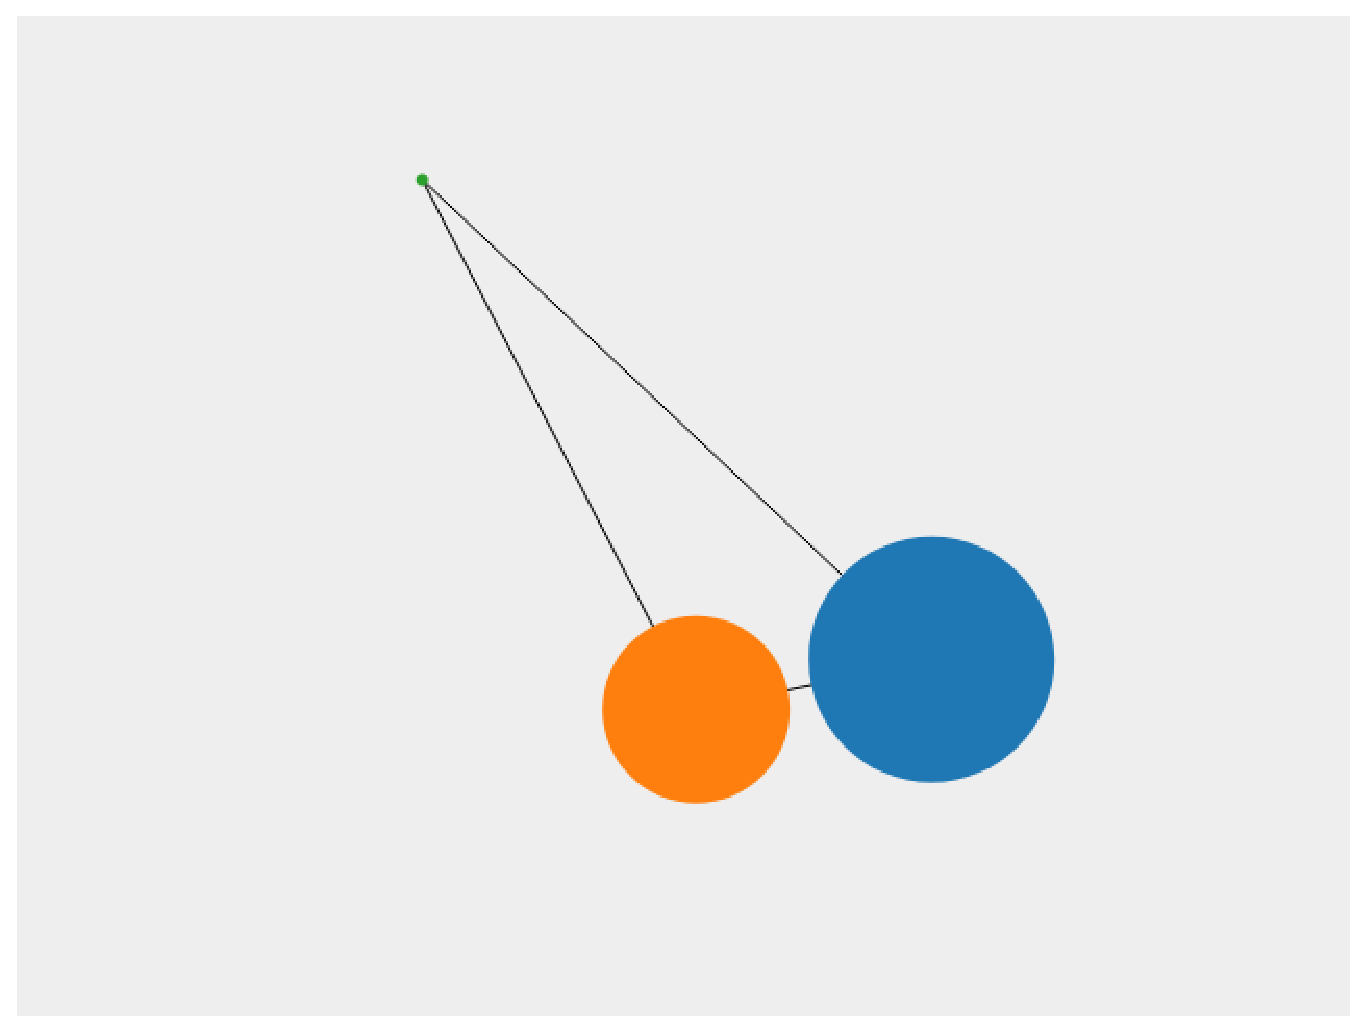
\includegraphics[width=0.4\textwidth]{img/cop-map-graph.eps}
  \caption{本システムによってプロジェクトメンバの関係性を可視化した様子}
  \label{cop-map-graph}
\end{figure}
